\documentclass[conference]{IEEEtran}
\usepackage[T1]{fontenc}
\usepackage[utf8]{inputenc}
\usepackage{graphicx}
\usepackage{amsmath,amssymb}
\usepackage{booktabs}
\usepackage{url}
\usepackage[hidelinks]{hyperref}

\title{CloudSentinel AI: A Context-Aware Framework for Cloud Misconfiguration Risk Assessment and Candidate Attack-Path Analysis}

\author{\IEEEauthorblockN{Harshith}}

\begin{document}
\maketitle

\begin{abstract}
Cloud Security Posture Management (CSPM) tools commonly report findings at the individual-resource level, which can obscure relationships among cloud assets and complicate remediation prioritisation. This paper proposes CloudSentinel AI, an AWS-focused framework for context-aware cloud misconfiguration assessment. The design collects selected configuration metadata, models assets and relationships in a knowledge graph, evaluates documented security rules, and derives candidate attack paths subject to explicit preconditions. A transparent contextual scoring heuristic is proposed to prioritise findings using asset criticality, exposure, identity permissions, data sensitivity, and graph context. An LLM-assisted reporting component is constrained to evidence-bounded, human-reviewed explanations and remediation recommendations. The paper also defines a controlled AWS evaluation protocol based on labelled scenarios. This work presents a framework and evaluation design; it does not claim completed experimental validation or general production effectiveness.
\end{abstract}

\begin{IEEEkeywords}
cloud security, cloud misconfiguration, AWS, knowledge graph, attack-path analysis, risk prioritisation, LLM-assisted security reporting
\end{IEEEkeywords}

\section{Introduction}
Cloud computing provides on-demand access to configurable computing resources \cite{nist2011cloud}, but security posture depends on the interaction of identities, network controls, storage policies, logging, and service relationships. An isolated configuration finding does not necessarily convey its operational context. For example, the priority of an exposed security group depends on the associated workload, reachable assets, privileges, and data sensitivity.

CloudSentinel AI is proposed as an AWS-focused research framework that combines configuration assessment with relationship-aware reasoning. The study follows a design-science approach in which the framework is the research artifact and the evaluation protocol tests its bounded claims \cite{hevner2004design}. Its intended contributions are: (i) an AWS resource-and-relationship model for a security knowledge graph, (ii) a candidate attack-path method that records explicit preconditions, (iii) a transparent contextual prioritisation heuristic, and (iv) an evidence-bounded LLM-assisted reporting workflow. The framework is a design proposal. Any claim of improved detection, prioritisation, or analyst effectiveness requires the controlled evaluation described in this paper.

\section{Background and Related Work}
Knowledge graphs provide a flexible representation for entities and their relationships \cite{hogan2021knowledge}. Attack-graph research has long used graph models to reason about possible sequences of security-relevant states \cite{sheyner2002automated,jha2002formal}. More recent cloud-focused work also illustrates the usefulness of graph reasoning for identifying critical paths in cloud tenants \cite{elmiger2023attackpaths}. These methods motivate relationship-aware analysis but do not remove the need to state attacker assumptions and validate path preconditions.

Cloud misconfiguration analysis is also important for identity controls. For example, anomalous AWS IAM policies can be identified through policy analysis \cite{vanede2022iam}. Explainability is an active cybersecurity research area \cite{rjoub2023xai}; however, generated natural-language text alone is not explainability. LLM-assisted output must be grounded in deterministic evidence and reviewed by a human, especially when it contains remediation advice \cite{xu2024llmcybersecurity}.

\section{Proposed Framework}
\subsection{Scope and Threat Model}
The initial scope is an AWS account containing EC2, S3, IAM, VPC/security-group, RDS, Secrets Manager, and CloudTrail configuration metadata. The framework assumes read-only collection credentials and evaluates only the resources made visible by those credentials. The threat model begins with an external or authenticated actor at a documented entry point and considers only transitions supported by collected configuration evidence. It does not assert an initial compromise, credential theft, exploit availability, or successful lateral movement unless those preconditions are explicitly represented and independently reviewed.

\subsection{Architecture and Graph Schema}
The proposed pipeline contains five stages. First, an asset collector retrieves versioned AWS metadata. Second, a configuration analyzer evaluates versioned rules derived from documented security guidance. Third, a graph builder represents assets and supported relationships as typed nodes and edges. Fourth, a candidate-path engine searches the graph under the threat model. Finally, a reporting component presents findings, path evidence, prioritisation rationale, and advisory remediation guidance. Table~\ref{tab:schema} defines the minimum graph schema.

\begin{figure}[t]
\centering
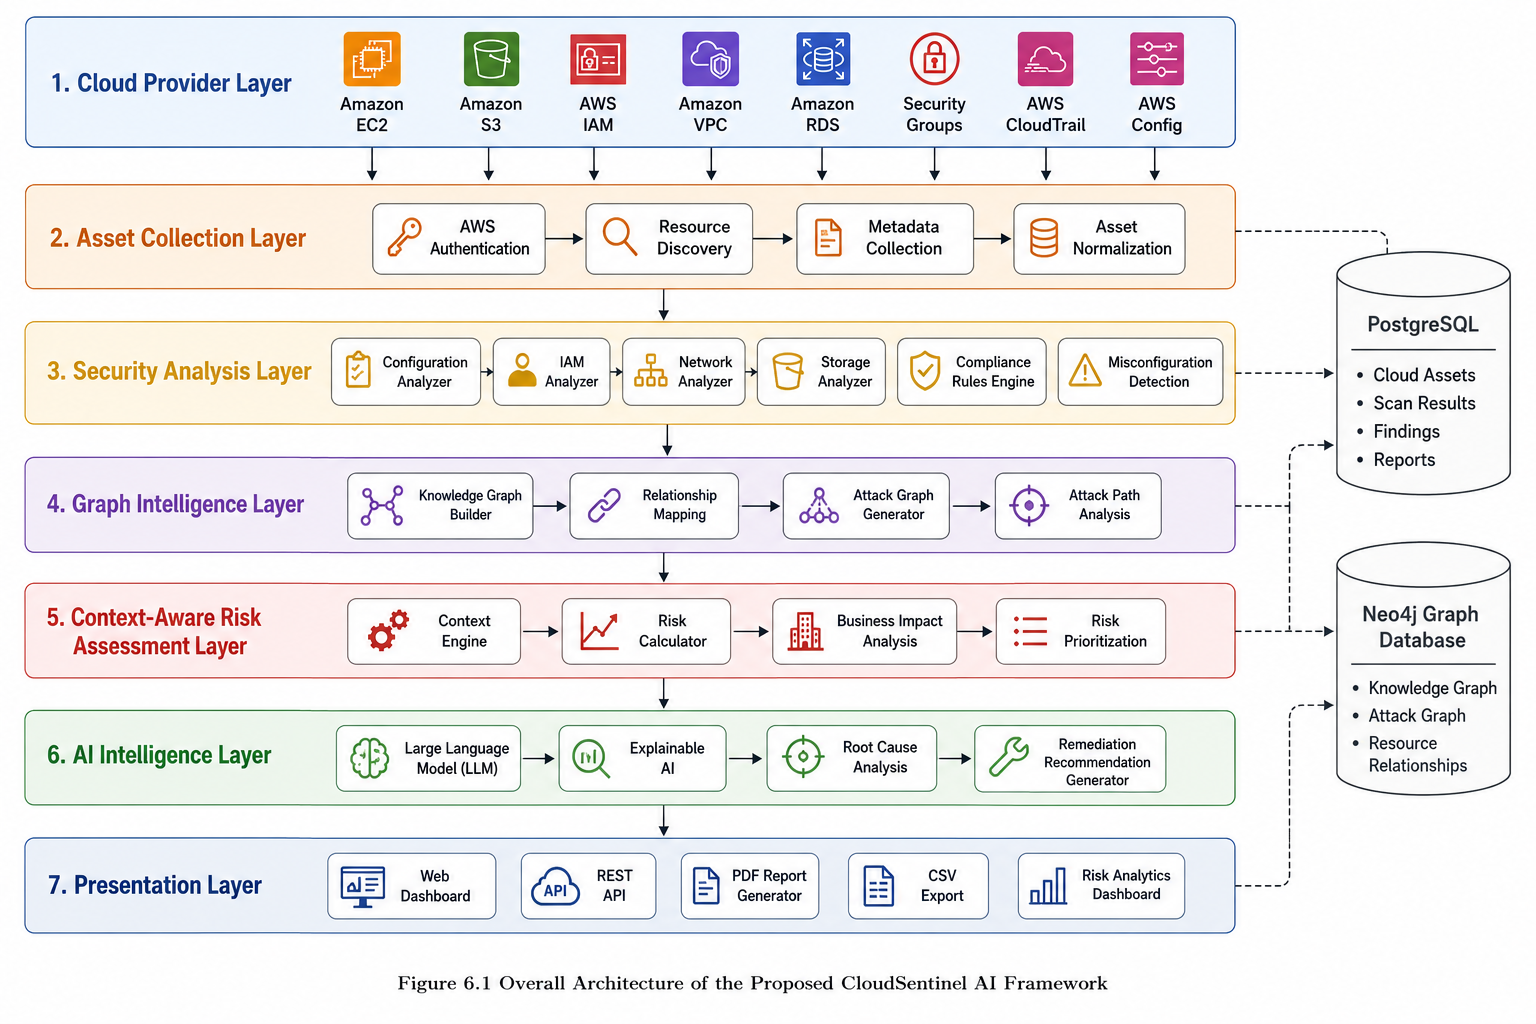
\includegraphics[width=\columnwidth,keepaspectratio]{../figures/image-6.1.png}
\caption{High-level CloudSentinel AI architecture. The figure illustrates the proposed pipeline; it is not an implementation-performance result.}
\label{fig:architecture}
\end{figure}

\begin{table}[t]
\caption{Minimum Proposed Graph Schema}
\label{tab:schema}
\centering
\footnotesize
\begin{tabular}{p{0.26\columnwidth} p{0.64\columnwidth}}
\toprule
Element & Required attributes or semantics \\
\midrule
Nodes & AWS resource, identity, policy, security finding, network boundary, or data asset; each has an account, region, source timestamp, and evidence identifier. \\
Edges & Typed relationship such as \emph{attached-to}, \emph{permits}, \emph{can-reach}, \emph{can-assume}, \emph{stores}, or \emph{has-finding}; every edge identifies its source metadata. \\
Findings & Rule identifier, affected node, observed evidence, severity mapping, and collection time. \\
Path record & Ordered edges, entry condition, required preconditions, target, supporting findings, and review status. \\
\bottomrule
\end{tabular}
\end{table}

\subsection{Candidate-Path Analysis and Prioritisation}
A graph edge represents a documented relationship or security-relevant condition; it does not independently prove exploitability. A candidate path is a bounded, loop-free sequence from a documented entry condition to a target asset. The engine will enumerate at most $k$ paths with a maximum depth $d$, reject paths with a missing required precondition, and retain evidence for every edge. It therefore performs bounded candidate-path discovery rather than claiming exhaustive enumeration of all attack paths.

The proposed prioritisation score is a transparent heuristic:
\begin{equation}
R = \alpha S + \beta C + \gamma P + \delta E,
\label{eq:risk}
\end{equation}
where all components are normalised to $[0,1]$: $S$ is documented finding severity, $C$ is asset criticality, $P$ is evidence-supported candidate-path context, and $E$ is externally reachable exposure. The non-negative weights sum to one and will be fixed before evaluation. Exposure is excluded from $C$ to avoid double counting. $R$ is a prioritisation score, not an estimated probability of compromise; sensitivity analysis will report how ranking changes under alternative weights.

\subsection{LLM-Assisted Reporting Contract}
The reporting component receives only approved, evidence-bounded findings, graph relationships, and remediation context. Each generated report must distinguish observed evidence from assumptions, identify missing preconditions, link each recommendation to relevant findings, and state that human review is required. Prompt engineering cannot guarantee accuracy or prevent hallucinations; the component is advisory and will be evaluated for evidence consistency, technical accuracy, clarity, and actionability. It must not automatically execute remediation or receive unapproved sensitive data.

\begin{table}[t]
\caption{Claim-to-Evidence Map for Evaluation}
\label{tab:claims}
\centering
\footnotesize
\begin{tabular}{p{0.28\columnwidth} p{0.57\columnwidth}}
\toprule
Claim & Required evaluation evidence and limitation \\
\midrule
Finding detection & Scenario ground truth, normalised scan output, and finding-level precision/recall; limited to selected rules and scenarios. \\
Candidate-path quality & Expected-path catalogue, edge evidence, and independent path review; graph connectivity alone is insufficient. \\
Prioritisation & Predefined reference ranking and sensitivity analysis; $R$ is a heuristic, not compromise probability. \\
LLM-assisted reporting & Human rubric for evidence consistency, accuracy, clarity, and actionability; output remains advisory. \\
\bottomrule
\end{tabular}
\end{table}

\section{Controlled Evaluation Design}
The proposed evaluation uses an isolated, authorised, non-production AWS account. All resources will be tagged, synthetic or non-sensitive data will be used, least-privilege roles and budget alarms will be configured, and every scenario will have a verified cleanup record. Intentionally weak configurations will remain within the defined laboratory boundary and will not be exposed to the public Internet.

\begin{table*}[t]
\caption{Controlled AWS Scenario Catalogue}
\label{tab:scenarios}
\centering
\begin{tabular}{p{0.08\textwidth} p{0.29\textwidth} p{0.53\textwidth}}
\toprule
ID & Scenario & Evaluation focus \\
\midrule
S1 & Public S3 storage exposure & Finding detection, evidence capture, and remediation guidance for a test-only bucket. \\
S2 & Overly permissive IAM policy & Detection of test-principal permissions and supported identity relationships. \\
S3 & Insecure network configuration & Detection of a laboratory security-group condition and documented reachability preconditions. \\
S4 & Disabled CloudTrail logging & Detection of an audit-logging condition and restoration recommendation. \\
S5 & Multi-stage candidate path & Evidence-backed relationship reasoning across test EC2, IAM, Secrets Manager, and S3 resources. \\
S6 & SSRF-to-IAM credential-access candidate path & Identification of configuration and identity preconditions in an instrumented, isolated test service; no public exposure or production credentials. \\
\bottomrule
\end{tabular}
\end{table*}

The evaluation distinguishes three units. A \emph{finding} is one rule violation attached to a resource. A \emph{candidate path} is an ordered graph sequence with documented preconditions. A \emph{consolidated alert} groups related findings for a shared path or asset context. Finding-level precision, recall, F1, false-positive rate, and false-negative rate will be calculated against scenario-specific ground truth. Candidate paths will be assessed as exact matches, partial matches, or invalid paths using an independently reviewed expected-path catalogue. LLM-generated reports will be assessed with a pre-defined rubric and human review.

CloudSentinel should be compared with selected baselines only under identical account scope, permissions, configuration, tool version, enabled checks, and execution date. Capability matrices based on vendor documentation must be labelled as documentation-based feature comparisons, not as benchmark performance results.

\section{Discussion and Limitations}
The proposed framework does not establish that a graph path is exploitable merely because related resources are connected. The threat model, evidence sources, path-validity rules, and score weights must be explicit. The controlled scenarios also do not represent all production environments, cloud providers, threat actors, or organisational policies. The initial scope is AWS only, and the in-memory graph design may not scale to large deployments without further engineering.

The LLM component adds cost, latency, privacy, and reliability concerns. It must not receive unapproved sensitive data, and its recommendations must not be executed automatically. These limitations motivate a staged evaluation in which each contribution is tied to an implementation artifact, metric, evidence source, and stated limitation.

\section{Conclusion}
This paper presented CloudSentinel AI, a proposed framework for combining AWS configuration assessment, knowledge-graph modeling, candidate attack-path analysis, contextual prioritisation, and LLM-assisted reporting. The central contribution is a reproducible evaluation design that separates labelled finding detection, candidate-path validity, prioritisation, and explanation quality. Future work will implement the pipeline, execute the controlled scenario catalogue, archive raw evidence, and report bounded results without generalising beyond the evaluated configurations.

\bibliographystyle{../IEEEtran}
\bibliography{../references}
\end{document}
